\chapter{Introduction}
\label{ch:introduction}

\section{What can Roslyn do?}
\label{sec:intro-what}

There are three major aspects that can be analyzed: the syntax, the semantic model and the data flow. 
The syntax, which is really just a collection of tokens that make up our source code, is the very basic level: no interpretation is done, we just make sure that the code that is written is valid syntactically. These validations are performed by confirming that the source code adheres to the rules specified in the C\# Language Specification\footnote{https://msdn.microsoft.com/en-us/library/ms228593.aspx}. Note however that there is no analyzing done of the actual meaning of these symbols thus far – we only determined that the textual representation is correct.
The next level facilitates this aspect: it interprets the semantic model. This means that so-called ‘symbols’ are created for each syntactical construct and represent a meaning. For example the following code will be interpreted as a class declaration (through the type ‘ClassDeclarationSyntax’)

\lstset{style=csharp, caption={Interpretation of a class declaration}}
\begin{lstlisting}
public class MyClass { }
\end{lstlisting}

	
while in this code, the ‘MyClass’ will be interpreted as an ‘IdentifierNameSyntax’:

   
\lstset{style=csharp, caption={Interpretation of an object instantiations}}
\begin{lstlisting}
var obj = new MyClass();
\end{lstlisting}  
	
This shows us that the semantic model knows the meaning of each syntactic construct regarding its context. This allows for more extensive analysis since we can now also analyze the relationship between specific symbols. 
Last but not least: the third aspect of source code that we can analyze is its data flow in a specific region. The ‘region’ here refers to either a method body or a field initializer. This tells us whether or a variable is read from/written to inside or outside the specified region, what the local variables in this region are, etc. This is a step above “simple” semantic analysis: rather than interpreting the meaning of a symbol in the code, we can now analyze how certain symbols are interacted with without actually executing the code itself.
For example consider the following method:

\lstset{style=csharp, caption={A method with definite assignments}}
\begin{lstlisting}
   public void MyMethod()
   {
      int x = 5;
      string y;
   }

\end{lstlisting}
	
Analyzing this method’s data flow and looking at the ‘DataFlowAnalysis.AlwaysAssigned’ property, would tell us that only 1 local here would be always assigned. However if we now alter the above code to this:

\lstset{style=csharp, caption={A method with conditional assignments}}
\begin{lstlisting}
   public void MyMethod()
   {
      int x = 5;
      string y;
      if(true)
         y = "My string";
   }
\end{lstlisting}
	
we now receive “2” as a result. This is an extremely powerful (albeit currently fairly limited) feature that allows us to actually interpret a code snippet’s data flow without executing it.


\section{Why was Roslyn built?}
\label{sec:intro-why}

Now that we know what Roslyn does it’s important to realize what gap is being closed. After all, something has to be special about Roslyn if it is to receive such widespread attention.

Roslyn introduced two very big changes to the community: the C\# compiler’s language changed and it has now become open-source. Prior to Roslyn, the C\# compiler was like a black box: everybody had access to the language specification so you could know what the rules of language were but the actual process of verifying your code against these rules was out of your reach. By open-sourcing Roslyn and placing it on CodePlex\footnote{https://roslyn.codeplex.com/} and afterwards Github\footnote{https://github.com/dotnet/roslyn/}, suddenly this box was opened and everybody could look at the internals of how a high-end compiler is written.

This brings us to the other big change: because Roslyn is written in C\# rather than C++, the C\# compiler is now able to bootstrap itself. This means that Roslyn can compile itself in C\# to compile the next versions of the Roslyn compiler! The process is simple: Roslyn is compiled using the old C++ compiler after which that newly created compiler re-compiles the Roslyn code base and suddenly you have a C\# compiler that is written in C\#. 
An added benefit of rewriting the compiler is the fact you can “discard” the older one. 

It should be noted here that Roslyn is also VB.NET its new compiler and as such, VB.NET-specific parts are written in VB.NET. You will also notice that every unit test that applies to both C\# and VB.NET is duplicated in both languages. In this paper, however, we will focus on the C\# aspects.

\section{Positivity of an open compiler}
\label{sec:intro-pos-comp}

Opening the compiler to the public brought a lot of good things, not in the least external contributions! Only 6 days after the Roslyn source was released, the first PR (Pull Request) was already integrated in the system!

\begin{figure}[h]
\centering
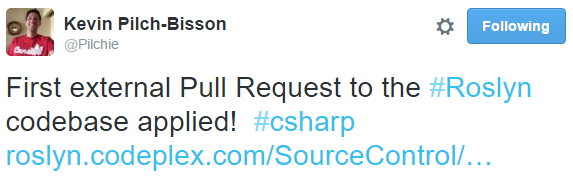
\includegraphics[scale=0.75]{roslyn-first-pr}
\caption[Announcement of the first PR by Kevin Pilch-Bisson]{Announcement of the first PR by Kevin Pilch-Bisson\protect\footnotemark}
\end{figure}

\footnotetext{https://twitter.com/pilchie/status/453968834408763392}

There are many more benefits to open-sourcing:

\begin{itemize}
	\item The amount of scrutiny the code goes through is greater now that the entire developer community has access to it.
	
	\item Developers themselves can now more easily learn how compilers work in a language they’re familiar with. Writing compilers has become more and more a “far-from-my-bed-show” with the rise of high-level languages – this might (re-)introduce some interest into such low-level concepts.
	
	\item It also facilitates advanced users by allowing them to inspect the bare bones of the compiler when something unexpected happens. Compilers are not bug free\footnote{http://stackoverflow.com/a/28820861/1864167}\footnote{http://stackoverflow.com/q/33694904/1864167} and implementations change over time\footnote{http://stackoverflow.com/a/30991931/1864167} which may lead to small but distinct differences in behaviour. An example that comes to mind is laid out in this Stack overflow question titled “Enums in lambda expressions are compiled differently; consequence of improvements?” where a user noticed that identical code compiles differently on the newer compiler version.
	
	\item Last but not least it simply provides a very robust and efficient parser that external parties now won’t have to develop themselves. This doesn’t necessarily mean that those tools should switch to the Roslyn platform but they might incorporate some ideas of it in their own parser (as is the case with ReSharper, a popular code-refactoring tool).\cite{Gorohovsky2014}

\end{itemize}


\section{Positivity of compiler APIs}
\label{sec:intro-pos-api}

Separately, providing APIs to your compiler brings benefits with it as well. Because of the broad support of APIs for all kinds of aspects of a compilation’s lifetime, a very convenient service is created where external parties can easily hook into and create their own diagnostics using the information that comes straight from the compiler. This encourages new tools aimed at the platform since the hassle of writing your own parser is removed – developers can go straight to implementing business logic. 

On top of that, the “native” support means that there is a seamless integration with Visual Studio, Microsoft’s own IDE\footnote{IDE: Integrated Development Environment, the editor in which you modify source files}. This integration allows you to use the results of your diagnostics to be displayed and used directly inside of Visual Studio rather than needing to build a third-party tool or a plugin.

This is the essence of why Roslyn is regarded as “Compiler as a Service”.



\section{Introduction to the paper}
\label{sec-intro-paper}

[TODO]